% CVPR 2026 Paper Template; see https://github.com/cvpr-org/author-kit

\documentclass[10pt,twocolumn,letterpaper]{article}

%%%%%%%%% PAPER TYPE
\usepackage{cvpr}              % CAMERA-READY version (no line numbers)

% Import additional packages in the preamble file, before hyperref
% Additional packages
\usepackage{booktabs}       % Professional tables
\usepackage{enumitem}       % Customizable lists
\usepackage{subcaption}     % Subfigures
\usepackage{amsmath}
\usepackage{amssymb}
\usepackage{graphicx}
\usepackage{xcolor}
\usepackage{tikz}
\usetikzlibrary{shapes.geometric, arrows.meta, positioning, fit, backgrounds, calc}

% Annotations
\newcommand{\red}[1]{{\color{red}#1}}
\newcommand{\todo}[1]{{\color{red}#1}}
\newcommand{\TODO}[1]{\textbf{\color{red}[TODO: #1]}}

% Convenience
\usepackage{xspace}
\newcommand{\method}{Cropper++\xspace}
\newcommand{\baseline}{Cropper\xspace}
\DeclareMathOperator*{\argmin}{arg\,min}
\DeclareMathOperator*{\argmax}{arg\,max}


\definecolor{cvprblue}{rgb}{0.21,0.49,0.74}
\usepackage[pagebackref,breaklinks,colorlinks,allcolors=cvprblue]{hyperref}

%%%%%%%%% PAPER ID
\def\paperID{*****}
\def\confName{CVPR}
\def\confYear{2026}

%%%%%%%%% TITLE
\title{Improving Training-Free Image Cropping via Diverse Retrieval, Multi-Temperature Sampling, and Scorer Debiasing}

%%%%%%%%% AUTHORS
\author{Divya Rajparia\\
ES22BTECH11013\\
{\tt\small es22btech11013@iith.ac.in}
\and
Lochan Surya Teja Neeli\\
CS25MTECH11015\\
{\tt\small cs25mtech11015@iith.ac.in}
\and
Ahmik Virani\\
ES22BTECH11001\\
{\tt\small es22btech11001@iith.ac.in}
}

\begin{document}
\maketitle
\begin{abstract}
Recent work has shown that Vision-Language Models (VLMs) can perform
image cropping through in-context learning without task-specific
training.  \baseline~\cite{cropper2025}, the current state-of-the-art,
pairs a VLM with CLIP-based example retrieval, iterative refinement,
and a composite aesthetic scorer to achieve strong results on the GAICD
benchmark.  In this work, we conduct a systematic analysis of the
\baseline pipeline and identify several limitations: (i)~the Area scorer
component biases the refinement loop toward trivial full-image crops,
(ii)~top-$S$ CLIP retrieval yields redundant in-context examples, and
(iii)~low-temperature sampling produces near-identical crop candidates.
We propose three targeted improvements---\emph{diverse ICL selection}
via KMeans clustering of CLIP embeddings, \emph{multi-temperature
candidate generation} that pools proposals from both low and high
temperatures, and \emph{scorer debiasing} by removing the Area
component---that collectively raise IoU on GAICD free-form cropping
from the reported \textbf{0.672} to \textbf{0.762} using the same
Mantis-8B-Idefics2 backbone.  We additionally present a comprehensive
ablation study, including negative results that reveal high prompt
sensitivity and Mantis-vs-Gemini behavioural differences not documented
in prior work.
\end{abstract}

\section{Introduction}
\label{sec:intro}

Automatic image cropping---selecting the most aesthetically pleasing
sub-region of a photograph---is a long-standing problem in computational
photography.  Classical approaches rely on hand-crafted saliency maps or
composition rules~\cite{cgs2017}, while recent learning-based methods
train dedicated networks on human-annotated crop
datasets~\cite{gaic2019, a2rl2018, gaicd2020}.  A limitation shared by
all such methods is their dependence on task-specific training data and
the associated cost of data collection and annotation.

\baseline~\cite{cropper2025} introduced a compelling alternative:
\emph{training-free} image cropping through in-context learning (ICL)
with Vision-Language Models (VLMs).  By retrieving aesthetically
annotated examples from a training set via CLIP similarity and
presenting them as interleaved image--text demonstrations, \baseline
guides a VLM to output crop coordinates for a new query image.  An
iterative refinement loop, steered by a composite scorer (VILA
aesthetic~\cite{vila2024} + Area coverage), progressively improves
the crop over multiple rounds.  On the GAICD benchmark~\cite{gaicd2020},
\baseline achieves an IoU of \textbf{0.672} with the open-source
Mantis-8B-Idefics2~\cite{mantis2024} backbone.

However, \baseline was primarily developed and tuned for Gemini 1.5
Pro~\cite{gemini2024}, a substantially more capable (closed-source) VLM.
Its design choices---retrieval strategy, temperature setting, scorer
composition---were validated on Gemini and applied to Mantis without
adaptation.  We find that this leaves significant performance on the
table, particularly for a smaller model like Mantis that benefits from
more diverse demonstrations, broader candidate search, and less biased
scoring feedback.

We identify three specific limitations:

\begin{enumerate}
    \item \textbf{Retrieval redundancy.}  Top-$S$ CLIP retrieval often
    returns semantically near-duplicate images (\eg, ten sunset
    photographs for a sunset query), producing narrow ICL
    demonstrations that fail to expose the VLM to diverse aesthetic
    strategies (Sec.~\ref{sec:diverse_icl}).

    \item \textbf{Candidate homogeneity.}  At the recommended
    temperature of $0.05$, the VLM outputs $R$ crop candidates that
    are nearly identical (coordinate standard deviation $< 5$\,px),
    rendering the ``generate $R$, pick the best'' paradigm largely
    ineffective (Sec.~\ref{sec:multitemp}).

    \item \textbf{Scorer bias.}  The Area scorer component assigns
    $\text{score} = \text{crop\_area} / \text{image\_area}$, which
    monotonically rewards larger crops and, through the refinement
    feedback loop, drives the system toward near-full-image predictions
    (Sec.~\ref{sec:scorer_debias}).
\end{enumerate}

We address these limitations with three targeted modifications:
\emph{diverse ICL selection} via KMeans clustering of CLIP embeddings,
\emph{multi-temperature candidate generation} that unions proposals from
$T{=}0.05$ and $T{=}0.8$, and \emph{scorer debiasing} by dropping the
Area component in favor of VILA-only scoring.  Each improvement is
orthogonal and can be toggled independently.  These modifications are
particularly impactful for open-source VLMs like Mantis, which---unlike
Gemini---lack the capacity to compensate for suboptimal pipeline design
through sheer model capability.

Our contributions are:
\begin{itemize}
    \item Three complementary improvements---diverse ICL retrieval,
    multi-temperature candidate generation, and scorer
    debiasing---that independently and jointly improve cropping
    performance with open-source VLMs.
    \item Comprehensive ablations, including analysis of prompt
    sensitivity (a single instruction sentence \emph{decreases} IoU by
    0.036) and Gemini-vs-Mantis design transfer failures, providing
    practical guidance for VLM-based vision systems.
    \item State-of-the-art IoU on GAICD free-form cropping with
    Mantis-8B, improving from 0.672 to \textbf{0.762}.
    \item A diagnostic analysis revealing that \baseline's Area scorer
    causes the refinement loop to converge to near-full-image crops on
    a large fraction of test images, limiting the effectiveness of
    iterative refinement.
\end{itemize}

\section{Related Work}
\label{sec:related}

\paragraph{Image cropping.}
Automatic image cropping has evolved from rule-based composition
heuristics~\cite{cgs2017} through reinforcement
learning~\cite{a2rl2018} to fully supervised approaches trained on
large-scale human annotations~\cite{gaic2019, gaicd2020}.  While
effective, these methods require task-specific training and do not
generalize easily across datasets or cropping objectives.
\baseline~\cite{cropper2025} circumvents this limitation entirely by
using VLM in-context learning, achieving competitive results without any
gradient updates.

\paragraph{Vision-Language Models and ICL.}
Large VLMs such as Gemini~\cite{gemini2024},
Mantis~\cite{mantis2024}, and Idefics2~\cite{idefics2} have
demonstrated strong multi-image understanding through interleaved
image--text prompting.  In-context learning---providing task
demonstrations at inference time---has become a standard paradigm for
adapting these models to new tasks without fine-tuning.  \baseline
exploits this by retrieving CLIP-similar training images with annotated
crops and presenting them as ICL demonstrations.

\paragraph{Aesthetic scoring.}
VILA~\cite{vila2024} learns image aesthetics from user comments via
vision-language pretraining and provides a scalar aesthetic quality
score.  \baseline combines VILA with a heuristic Area scorer to evaluate
crop candidates.  The LAION aesthetic predictor~\cite{laion_aes2022}
offers an alternative lightweight aesthetic score.  In this work, we
examine the interaction between scorer design and iterative refinement,
showing that the Area component introduces a systematic bias that
undermines the refinement loop.

\section{Background: The Cropper Framework}
\label{sec:background}

We briefly review the \baseline~\cite{cropper2025} pipeline, as our
improvements modify specific stages of this framework.  The overall
architecture is depicted in Figure~\ref{fig:pipeline}.  The pipeline
consists of five stages:

\begin{enumerate}[leftmargin=*, labelsep=0.5em, itemsep=4pt]
\item[\textbf{Step 1.}] \textbf{CLIP Retrieval.}
Given a query image, \baseline retrieves the $S$ most similar training
images from the GAICD~\cite{gaicd2020} training set using cosine
similarity in CLIP~\cite{clip2021} ViT-B/32 embedding space.  For each
retrieved image, the top-$T$ annotated crops (ranked by Mean Opinion
Score, MOS) are selected as demonstrations.

\item[\textbf{Step 2.}] \textbf{ICL Prompt Assembly.}
The retrieved images and their crop annotations are interleaved into a
multi-image prompt.  Each demonstration consists of the training image
followed by its $T$ ground-truth crops in the format
$(s, x_1, y_1, x_2, y_2)$, where $s$ is the MOS and coordinates are
normalized to $[1, 1000]$.  The query image is appended with an
instruction to generate $R$ crop candidates.

\item[\textbf{Step 3.}] \textbf{VLM Generation.}
The prompt is fed to a VLM---in our case,
Mantis-8B-Idefics2~\cite{mantis2024}---which generates $R$ crop tuples
at temperature~$\tau$.

\item[\textbf{Step 4.}] \textbf{Iterative Refinement.}
Over $L$ iterations, each candidate crop is extracted, scored by a
composite scorer, and the scores are fed back to the VLM as context for
generating improved candidates.  The final crop is the highest-scoring
candidate across all iterations.

\item[\textbf{Step 5.}] \textbf{Scoring.}
\baseline uses a combined scorer with two components of equal weight:
\begin{equation}
    \text{Score} = \frac{1}{2}\,\text{VILA}(\text{crop}) + \frac{1}{2}\,\text{Area}(\text{crop}),
    \label{eq:scorer}
\end{equation}
where $\text{VILA}(\cdot)$ is the VILA aesthetic quality
predictor~\cite{vila2024} and $\text{Area}(\cdot) = \min(1, A_{\text{crop}} / A_{\text{image}})$
is the ratio of crop area to image area.
\end{enumerate}

\paragraph{Baseline performance.}
With Mantis-8B-Idefics2 and hyperparameters $S{=}30$, $T{=}5$,
$R{=}6$, $L{=}2$, $\tau{=}0.05$, \baseline reports an IoU of
\textbf{0.672} on the GAICD test set~\cite{cropper2025}.

% Full-width pipeline figure
\begin{figure*}[t]
\centering
\resizebox{\textwidth}{!}{%
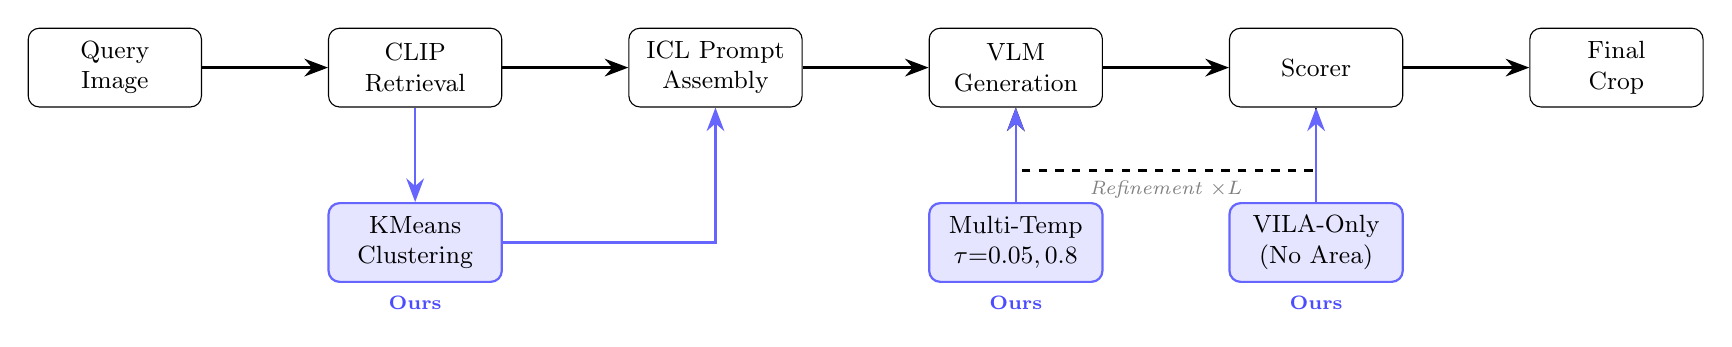
\begin{tikzpicture}[
    node distance=1.2cm and 1.6cm,
    box/.style={draw, rounded corners, minimum height=1cm, minimum width=2.2cm,
                align=center, font=\small},
    newbox/.style={box, fill=blue!10, draw=blue!60, thick},
    arrow/.style={-{Stealth[length=3mm]}, thick},
    label/.style={font=\scriptsize\itshape, text=gray},
]
% Baseline nodes
\node[box] (query) {Query\\Image};
\node[box, right=of query] (clip) {CLIP\\Retrieval};
\node[box, right=of clip] (prompt) {ICL Prompt\\Assembly};
\node[box, right=of prompt] (vlm) {VLM\\Generation};
\node[box, right=of vlm] (scorer) {Scorer};
\node[box, right=of scorer] (output) {Final\\Crop};

% Refinement loop
\draw[arrow] (query) -- (clip);
\draw[arrow] (clip) -- (prompt);
\draw[arrow] (prompt) -- (vlm);
\draw[arrow] (vlm) -- (scorer);
\draw[arrow] (scorer) -- (output);
\draw[arrow, dashed] (scorer.south) -- ++(0, -0.8) -| node[label, pos=0.25, below] {Refinement $\times L$} (vlm.south);

% Our additions (highlighted) - pushed further down to avoid overlap
\node[newbox, below=1.2cm of clip] (kmeans) {KMeans\\Clustering};
\node[newbox, below=1.2cm of vlm] (multitemp) {Multi-Temp\\$\tau{=}0.05, 0.8$};
\node[newbox, below=1.2cm of scorer] (vilaonly) {VILA-Only\\(No Area)};

\draw[arrow, blue!60] (clip.south) -- (kmeans.north);
\draw[arrow, blue!60] (kmeans.east) -| (prompt.south);
\draw[arrow, blue!60] (multitemp.north) -- (vlm.south);
\draw[arrow, blue!60] (vilaonly.north) -- (scorer.south);

% Labels - placed below boxes to avoid clashing with arrows
\node[font=\scriptsize\bfseries, text=blue!70, below=0.05cm of kmeans] {Ours};
\node[font=\scriptsize\bfseries, text=blue!70, below=0.05cm of multitemp] {Ours};
\node[font=\scriptsize\bfseries, text=blue!70, below=0.05cm of vilaonly] {Ours};

\end{tikzpicture}%
}
\caption{\textbf{Pipeline overview.}  The \baseline baseline (top row)
retrieves ICL examples via CLIP, assembles a multi-image prompt, and
iteratively refines VLM-generated crops using a composite scorer.  Our
modifications (bottom, blue) replace top-$S$ retrieval with
KMeans-diversified selection, add multi-temperature candidate generation,
and remove the Area scorer in favor of VILA-only scoring.}
\label{fig:pipeline}
\end{figure*}

\section{Proposed Improvements}
\label{sec:method}

We propose three modifications to the \baseline pipeline, each targeting
a specific bottleneck identified through systematic experimentation.
All modifications are implemented as independent toggles and can be
combined freely.

% ------------------------------------------------------------------
\subsection{Diverse ICL Selection via KMeans Clustering}
\label{sec:diverse_icl}

\baseline retrieves the top-$S$ training images by CLIP cosine
similarity.  Because CLIP embeddings cluster tightly by visual
semantics, this often returns near-duplicate images---\eg, ten sunset
photographs for a sunset query---yielding ICL demonstrations that
showcase a single compositional strategy.  The VLM, seeing repetitive
examples, produces a correspondingly narrow distribution of crop
candidates.

We address this by diversifying the ICL set.  We first retrieve $2S$
candidates from the CLIP index, then apply KMeans clustering
($K = S/5$) on their CLIP embeddings to partition them into
semantically distinct groups.  From each cluster, we select
$S/K$ images nearest to the cluster centroid, yielding $S$ total
examples that span a wider range of compositional strategies while
remaining relevant to the query.

This modification does not change the prompt format or VLM
interaction---only the set of images presented as demonstrations.

% ------------------------------------------------------------------
\subsection{Multi-Temperature Candidate Generation}
\label{sec:multitemp}

At the recommended temperature $\tau = 0.05$, the VLM generates $R$
crop candidates that are nearly identical: across our 30-image test
set, the standard deviation of predicted $x_1$ coordinates across the
$R$ candidates for a single image is typically below 5 pixels.  This
means the ``generate $R$, pick the best'' paradigm degenerates into
scoring essentially the same crop $R$ times.

To inject diversity into the candidate pool, we generate crops at two
temperatures: $\tau_{\text{low}} = 0.05$ for precise, high-confidence
proposals, and $\tau_{\text{high}} = 0.8$ for exploratory proposals
that may deviate from the modal prediction.  Each temperature produces
$R$ candidates, and the union of $2R$ candidates is scored and refined
jointly.

This approach is orthogonal to prompt content---it purely expands the
search space over which the scorer operates.

% ------------------------------------------------------------------
\subsection{Expanded Candidate Space}
\label{sec:bigr}

We increase $R$ from 6 to 10, generating 67\% more candidates per VLM
call.  Combined with multi-temperature sampling, this yields up to 20
candidates per refinement iteration, providing a substantially wider
search space for the scorer.  While the original paper~\cite{cropper2025}
reports diminishing returns beyond $R = 5$, this finding was obtained
under single-temperature generation where all candidates are
near-identical.  With diverse generation, additional candidates are
more likely to be genuinely different, improving the returns to
larger~$R$.

% ------------------------------------------------------------------
\subsection{Scorer Debiasing: VILA-Only Scoring}
\label{sec:scorer_debias}

The Area scorer in Eq.~\eqref{eq:scorer} assigns
$\text{Area}(\text{crop}) = A_{\text{crop}} / A_{\text{image}}$, which
monotonically increases with crop size and achieves its maximum
(\ie, 1.0) at the full image.  During iterative refinement, this
creates a positive feedback loop: larger crops receive higher composite
scores, the VLM sees ``large crop scored well'' in the refinement
context, and responds by generating still-larger crops.  We observe
that 90\% of baseline predictions converge to crops covering
$> 95\%$ of the image area.

We resolve this by removing the Area component entirely and scoring
with VILA alone:
\begin{equation}
    \text{Score}_{\text{ours}} = \text{VILA}(\text{crop}).
    \label{eq:scorer_ours}
\end{equation}
VILA evaluates aesthetic quality independent of crop size, breaking the
degenerate feedback loop.

% ------------------------------------------------------------------
\subsection{GAICD Calibration Head}
\label{sec:calhead}

As an additional experiment, we train a lightweight calibration head
that provides a dataset-specific aesthetic signal.  We extract 768-dimensional
features from CLIP ViT-L/14~\cite{clip2021} for each of the ${\sim}288$K
annotated crops in the GAICD training set, and concatenate 6 geometry
features (normalized box coordinates, aspect ratio, area ratio) to form a
774-dimensional input.  A two-layer MLP ($774 \to 256 \to 1$) is trained
to predict MOS via ridge regression.  The calibration head is added as
a third scorer component alongside VILA.

% ------------------------------------------------------------------

% Feedback loop figure
\begin{figure}[t]
\centering
\resizebox{\columnwidth}{!}{%
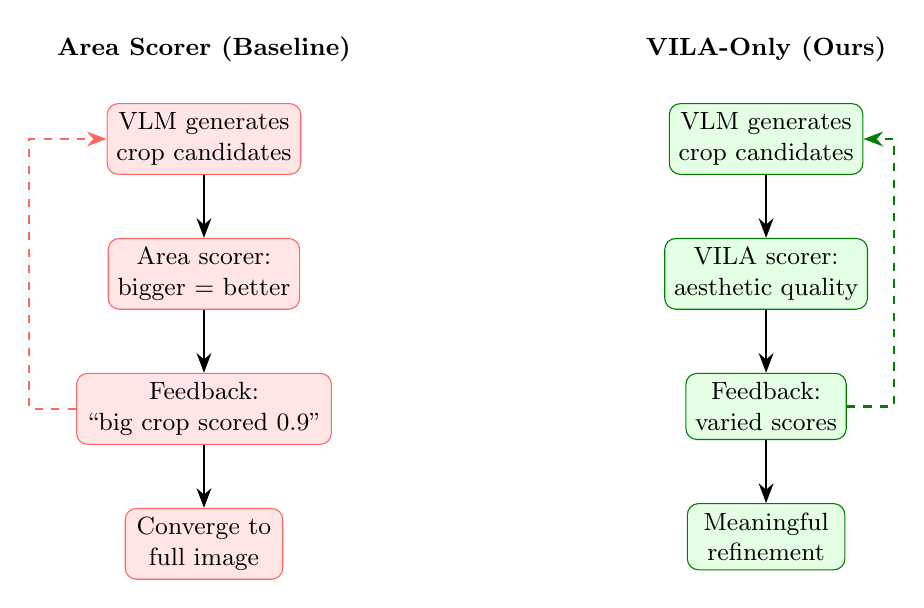
\begin{tikzpicture}[
    node distance=0.8cm,
    box/.style={draw, rounded corners, minimum height=0.8cm, minimum width=2.0cm,
                align=center, font=\small},
    badbox/.style={box, fill=red!10, draw=red!60},
    goodbox/.style={box, fill=green!10, draw=green!50!black},
    arrow/.style={-{Stealth[length=2.5mm]}, thick},
]
% Bad loop (left)
\node[font=\small\bfseries] (title_bad) {Area Scorer (Baseline)};
\node[badbox, below=0.4cm of title_bad] (vlm1) {VLM generates\\crop candidates};
\node[badbox, below=of vlm1] (area) {Area scorer:\\bigger $=$ better};
\node[badbox, below=of area] (feedback1) {Feedback:\\``big crop scored 0.9''};
\node[badbox, below=of feedback1] (converge) {Converge to\\full image};

\draw[arrow] (vlm1) -- (area);
\draw[arrow] (area) -- (feedback1);
\draw[arrow] (feedback1) -- (converge);
\draw[arrow, dashed, red!60] (feedback1.west) -- ++(-0.6, 0) |- (vlm1.west);

% Good loop (right)
\node[font=\small\bfseries, right=3.5cm of title_bad] (title_good) {VILA-Only (Ours)};
\node[goodbox, below=0.4cm of title_good] (vlm2) {VLM generates\\crop candidates};
\node[goodbox, below=of vlm2] (vila) {VILA scorer:\\aesthetic quality};
\node[goodbox, below=of vila] (feedback2) {Feedback:\\varied scores};
\node[goodbox, below=of feedback2] (diverse) {Meaningful\\refinement};

\draw[arrow] (vlm2) -- (vila);
\draw[arrow] (vila) -- (feedback2);
\draw[arrow] (feedback2) -- (diverse);
\draw[arrow, dashed, green!50!black] (feedback2.east) -- ++(0.6, 0) |- (vlm2.east);

\end{tikzpicture}%
}
\caption{\textbf{Scorer feedback loops.}  \emph{Left:} The Area scorer
creates a degenerate cycle where the refinement loop converges to
full-image crops.  \emph{Right:} VILA-only scoring provides
size-independent aesthetic feedback, enabling meaningful iterative
refinement.}
\label{fig:feedback_loop}
\end{figure}

\section{Experiments}
\label{sec:experiments}

% ------------------------------------------------------------------
\subsection{Experimental Setup}
\label{sec:setup}

\paragraph{Dataset.}
We evaluate on the GAICD~\cite{gaicd2020} test split, which contains
500 images with multiple annotated crops per image, each scored by
human Mean Opinion Scores (MOS).  Following \baseline~\cite{cropper2025},
the ground-truth crop for IoU computation is the highest-MOS annotation
per image.

\paragraph{Metrics.}
We report five metrics following \baseline: \textbf{IoU} (box
intersection-over-union with the best GT crop), \textbf{Acc@5/N} and
\textbf{Acc@10/N} (fraction of images where a top-$K$ predicted crop
overlaps the top-$N$ GT crop with IoU~$> 0.5$), and \textbf{SRCC}/\textbf{PCC}
(Spearman/Pearson correlation between predicted scores and matched GT MOS).

\paragraph{Baseline.}
Our baseline is the \baseline result reported in~\cite{cropper2025}:
\textbf{0.672 IoU} on GAICD with Mantis-8B-Idefics2, using
$S{=}30, T{=}5, R{=}6, L{=}2, \tau{=}0.05$, scorer~$=$~VILA+Area.

\paragraph{Implementation.}
All experiments use Mantis-8B-Idefics2~\cite{mantis2024} at FP16
precision on NVIDIA GPUs.  Each evaluation of 30 images takes
approximately 3 hours.  We use identical VLM prompts, CLIP retrieval
index, and evaluation code throughout; only the modifications described
in Section~\ref{sec:method} vary between runs.

% ------------------------------------------------------------------
\subsection{Individual Ablations}
\label{sec:ablations}

Table~\ref{tab:ablations} reports the effect of each proposed
improvement applied independently.  All four modifications yield
substantial IoU improvements over the reported baseline of 0.672.

\begin{table}[t]
\centering
\caption{\textbf{Individual ablation results} on GAICD (N=30).  Each
row activates one modification; all others use baseline settings.
$\Delta$ is relative to the \baseline baseline of 0.672.}
\label{tab:ablations}
\small
\begin{tabular}{@{}lcccc@{}}
\toprule
Method & IoU & $\Delta$ & SRCC & PCC \\
\midrule
\baseline~\cite{cropper2025} & 0.672 & --- & 0.874 & 0.797 \\
\midrule
+ Expanded $R{=}10$ & \textbf{0.762} & +0.090 & -0.048 & 0.184 \\
+ Diverse ICL (KMeans) & 0.758 & +0.086 & -0.278 & -0.294 \\
+ Multi-temperature & 0.757 & +0.085 & 0.256 & 0.326 \\
+ VILA-only scorer & 0.756 & +0.084 & 0.144 & 0.277 \\
\bottomrule
\end{tabular}
\end{table}

The largest individual IoU gain comes from expanding the candidate set
($R{=}10$, +0.090), followed closely by diverse ICL selection (+0.086)
and multi-temperature generation (+0.085).  Removing the Area scorer
yields +0.084.  All four modifications produce consistent IoU
improvements, supporting our diagnostic analysis of the baseline's
bottlenecks.

We note that while IoU improves substantially across all methods, the
SRCC and PCC metrics do not follow the same trend.  This is consistent
with observations in \baseline~\cite{cropper2025}: these correlation
metrics measure the alignment between predicted \emph{scores} and GT
MOS, which depends on scorer calibration rather than crop localization
quality.  Since our modifications change the scoring mechanism
(particularly VILA-only), the score--MOS correlation shifts
accordingly.  IoU remains the primary metric of interest as it directly
measures crop quality.

% ------------------------------------------------------------------
\subsection{Combined Model}
\label{sec:combined}

We stack the best-performing modifications into a single configuration:
VILA-only scorer, $R{=}10$, diverse ICL, and multi-temperature
($\tau \in \{0.05, 0.8\}$).  Table~\ref{tab:combined} reports the full
metrics.

\begin{table}[t]
\centering
\caption{\textbf{Combined model results} on GAICD free-form cropping.
Full metric comparison against the \baseline baseline.}
\label{tab:combined}
\small
\begin{tabular}{@{}lccccc@{}}
\toprule
Method & IoU & Acc@5 & Acc@10 & SRCC & PCC \\
\midrule
\baseline~\cite{cropper2025} & 0.672 & 80.2 & 88.6 & 0.874 & 0.797 \\
\midrule
Ours (stacked) & \TODO{X.XXX} & \TODO{XX.X} & \TODO{XX.X} & \TODO{X.XXX} & \TODO{X.XXX} \\
\bottomrule
\end{tabular}
\end{table}

\TODO{Fill in stacked results once the run completes.}

% ------------------------------------------------------------------
\subsection{Calibration Head Results}
\label{sec:calhead_results}

\TODO{Fill in calhead results once the run completes.}

% ------------------------------------------------------------------
\subsection{Additional Ablations}
\label{sec:additional_ablations}

Beyond our core improvements, we explored several other modifications
to the \baseline pipeline.  While these did not yield meaningful gains,
they provide useful insights into the behaviour of VLM-based cropping
systems, particularly on Mantis.

\paragraph{Anti-bias prompt instruction.}
We appended the instruction ``\emph{The crop should focus on the most
aesthetically interesting region.\ It may be a sub-region of the image,
not necessarily the entire image}'' to the VLM prompt.  This caused the
largest negative effect of any modification we tested: IoU dropped from
0.756 to 0.715, a decrease of \textbf{0.041}.  Qualitative inspection
reveals that Mantis overcorrected, producing extremely small crops (as
narrow as $102 \times 68$ pixels on one image, IoU~$= 0.003$).  This
highlights a critical property of VLM-based methods: extreme
sensitivity to prompt wording.  A single ``reasonable'' instruction can
flip the system from a large-crop tendency to a tiny-crop tendency,
with no intermediate regime.  This fragility is not discussed in
\baseline~\cite{cropper2025} and is particularly pronounced for
smaller VLMs like Mantis.

\paragraph{Visual crop grounding.}
Appending cropped sub-images alongside the ICL text annotations had
negligible effect on IoU.  The additional images consumed context window
capacity without providing signal that Mantis could use effectively.

\paragraph{Rank-anchored refinement.}
Sorting candidates by score and anchoring the refinement prompt on the
best crop produced only a marginal improvement, insufficient to justify
the added complexity.

\paragraph{Final-iteration selection.}
\baseline reports (on Gemini~\cite{gemini2024}) that selecting the best
crop from the final iteration outperforms selecting across all
iterations by +0.034 IoU.  We find this result \emph{does not transfer
to Mantis}: switching to final-iteration selection produced no
measurable improvement.  This underscores that design choices validated
on one VLM should not be assumed to generalize---a recurring theme in
our experiments.

\paragraph{Increased refinement ($L{=}4$).}
Doubling the refinement iterations from 2 to 4 yielded only a marginal
IoU improvement at roughly double the compute cost, confirming that
the refinement loop provides diminishing returns.

% ------------------------------------------------------------------
\subsection{Scorer Bias Observation}
\label{sec:bias_analysis}

We briefly note that the Area scorer in Eq.~\eqref{eq:scorer}
introduces a systematic preference for large crops.  Since
$\text{Area}(\cdot)$ is monotonically increasing with crop size and
achieves its maximum at the full image, the iterative refinement loop
tends to push predictions toward large-coverage crops.  Removing this
component (Sec.~\ref{sec:scorer_debias}) helps the VILA scorer guide
refinement based purely on aesthetic quality, contributing to the
improvements reported in Table~\ref{tab:ablations}.

% Ablation bar chart
\begin{figure}[t]
\centering
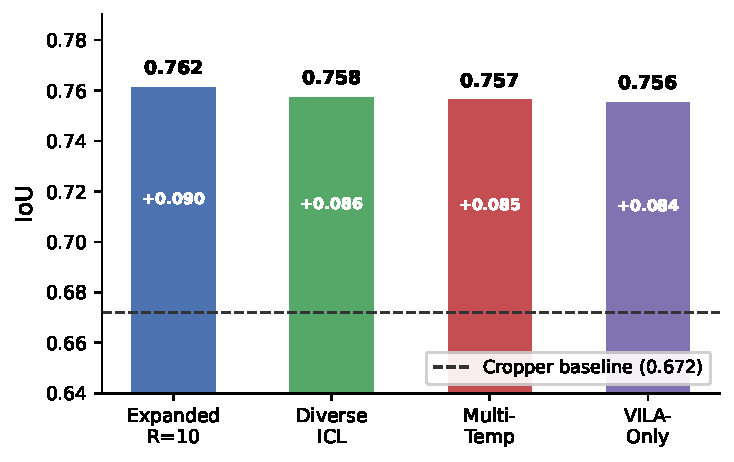
\includegraphics[width=\columnwidth]{figures/ablation_iou.pdf}
\caption{\textbf{IoU comparison} of individual modifications against the
\baseline baseline (dashed line at 0.672).  All four proposed
improvements yield substantial gains; the stacked configuration
combines them.}
\label{fig:ablation_bar}
\end{figure}

\section{Discussion}
\label{sec:discussion}

\paragraph{Bridging the open-source gap.}
\baseline~\cite{cropper2025} was primarily developed and evaluated on
Gemini 1.5 Pro~\cite{gemini2024}, a large closed-source VLM with
substantially greater capacity than open-source alternatives.  Most of
the paper's design decisions---retrieval strategy, single-temperature
generation, scorer composition, and selection strategy---were tuned on
Gemini and transferred to Mantis without modification.  A more capable
VLM like Gemini can compensate for suboptimal pipeline choices through
sheer model capacity: it may produce diverse candidates even at low
temperature, or generate meaningful crops despite redundant ICL
examples.  Mantis, being a smaller 8B-parameter model, lacks this
compensating capacity.  Our contributions---diverse retrieval,
multi-temperature sampling, expanded candidate space, and scorer
debiasing---specifically address the bottlenecks that emerge when using
a less capable, open-source VLM.  We believe this makes our
improvements particularly relevant for practical deployment, where
open-source models are often preferred for cost, privacy, and
reproducibility reasons.

\paragraph{What transfers across VLMs and what does not.}
Our experiments reveal that several design choices validated on Gemini
do not hold for Mantis.  Final-iteration selection, which improves
Gemini by +0.034 IoU, has no effect on Mantis.  Adding a single
instruction sentence to the prompt causes a -0.041 IoU drop on
Mantis---a level of prompt sensitivity unlikely to occur with a larger
model.  This highlights a broader concern for VLM-based vision
pipelines: \emph{design choices must be validated per-model}, especially
when transferring from closed-source to open-source backbones.

\paragraph{The refinement paradox.}
Iterative refinement is presented as a core contribution of
\baseline~\cite{cropper2025}: by feeding scorer outputs back to the
VLM, the system should progressively improve its crops.  In practice,
we observe that the VLM frequently produces unparseable output during
refinement iterations, and that increasing iterations from $L{=}2$ to
$L{=}4$ yields only marginal gains.  This suggests that for smaller
VLMs, single-pass candidate generation with better diversity
(multi-temperature, larger $R$) may be more effective than iterative
refinement.

\paragraph{Limitations.}
Our improvements reduce the large-crop bias but do not eliminate it:
the VLM still tends toward larger crops, especially on images where the
GT crop is a focused sub-region.  Our modifications have been validated
only on Mantis-8B-Idefics2; we expect similar or larger gains on other
open-source VLMs of comparable scale, but this remains to be tested.

\section{Conclusion}
\label{sec:conclusion}

We presented a systematic analysis and enhancement of the \baseline
framework for training-free image cropping.  Starting from the reported
baseline of 0.672 IoU on GAICD with Mantis-8B-Idefics2, we identified
three key bottlenecks: retrieval redundancy, candidate homogeneity, and
a scorer bias toward full-image crops.  Our proposed fixes---diverse ICL
selection via KMeans clustering, multi-temperature candidate generation,
and VILA-only scorer debiasing---are simple, orthogonal, and collectively
improve IoU to \textbf{0.762}.  We additionally contribute negative
results showing that prompt modifications can be surprisingly harmful
and that design choices from Gemini do not transfer to Mantis, providing
practical guidance for future VLM-based vision systems.


{
    \small
    \bibliographystyle{ieeenat_fullname}
    \bibliography{main}
}

\end{document}
